% $Id: TimeMgr_desdoc.tex,v 1.1 2002/08/18 22:43:36 eschwab Exp $

\documentclass[]{article}

\usepackage{epsf}
\usepackage{html}
\usepackage[T1]{fontenc}
\usepackage[dvips]{graphics,color}

\textwidth 6.5in
\textheight 8.5in
\addtolength{\oddsidemargin}{-.75in}

\begin{document}

\bodytext{BGCOLOR=white LINK=#083194 VLINK=#21004A}

\begin{titlepage}

\begin{center}
{\Large Earth System Modeling Framework } \\
\vspace{.25in}
{\Large {\bf Time Manager Design}} \\
\vspace{.25in}
{\large {\it Earl Schwab}} \\
\vspace{.25in}
{August 16, 2002}
\vspace{.5in}
\end{center}

\begin{latexonly}
\vspace{5.5in}
\begin{tabular}{p{5in}p{.9in}}
\hrulefill \\
\noindent {\bf NASA Earth Science Technology Office} \\
\noindent Computational Technologies Project \\
\noindent CAN 00-OES-01 \\
\noindent http://www.esmf.ucar.edu \\
\end{tabular}
\end{latexonly}

\end{titlepage}

\tableofcontents

\newpage
\section{Synopsis}
% $Id: TimeMgr_syn.tex,v 1.2 2003/02/11 18:58:56 eschwab Exp $

%\section{Synopsis}

The Earth System Modeling Framework (ESMF) Time Management Library
provides utilities for time and date representation and calculation,
and higher-level utilities that control model time stepping and alarming.
It is designed to meet the requIeements as specified in the ESMF 
Requirements document~\ref{esmf_req<<fixme>>}.


\section{Object Model}
% $Id: TimeMgr_obj1.tex,v 1.4 2003/08/12 14:32:50 cdeluca Exp $

\subsection{Object Model}

The core Time Manager Library consists of six object-oriented classes (types)
organized in four layers of inheritance, aggregation and composition,
as shown in Figure 1 below.  The primary classes intended for
direct model use are:

\begin{itemize}
\item {\tt ESMF\_TimeInterval}
\item {\tt ESMF\_Time}
\item {\tt ESMF\_Clock}
\item {\tt ESMF\_Alarm}
\item {\tt ESMF\_Calendar}
\end{itemize}

These directly correspond to, and encapsulate the representation and
behavior of, Time Intervals, Time instants, Clocks, Alarms, and Calendars,
as specified in the ESMF Time Manager Requirements document.
{\tt ESMF\_TimeInterval} is independent of any calendar (except when used
as a Calendar interval), whereas {\tt ESMF\_Time} is dependent on a calendar
type, such as Gregorian or Julian.  Multiple objects of all these primary
classes can be instantiated within a single application.

There is also one secondary supporting class, not intended for direct
use in model applications.  This is {\tt ESMF\_BaseTime}.  {\tt ESMF\_BaseTime}
serves as the base class for both {\tt ESMF\_TimeInterval} and
{\tt ESMF\_Time},capturing common core time representation and functionality.

{\tt ESMF\_Calendar} encapsulates all the required calendar types and behavior,
isolating them from Time instants.  Specific calendar-type objects (e.g.
Gregorian, Julian, no-leap, etc.) can be instantiated from {\tt ESMF\_Calendar}.
Ideally, for a given application, no more than one calendar
object should be instantiated for each calendar type.  The idea is that
a calendar object is analogous to a "wall calendar," serving as a single
point of reference throughout an application.  For example, a single
Gregorian calendar can be instantiated within an application and shared
among all the time instants.  However, the design does not preclude having
multiple calendar instantiations.  For practical reasons of using SPMD or
MPMD application execution models, there may be multiple instantiations
of a calendar type; for example, one per component.

For object integrity, all class data members are private; access is via
public member functions only. The entire {\tt ESMF\_BaseTime} base class
will be "protected," so that it can only be inherited; it will not be directly
instantiable.

\begin{center}
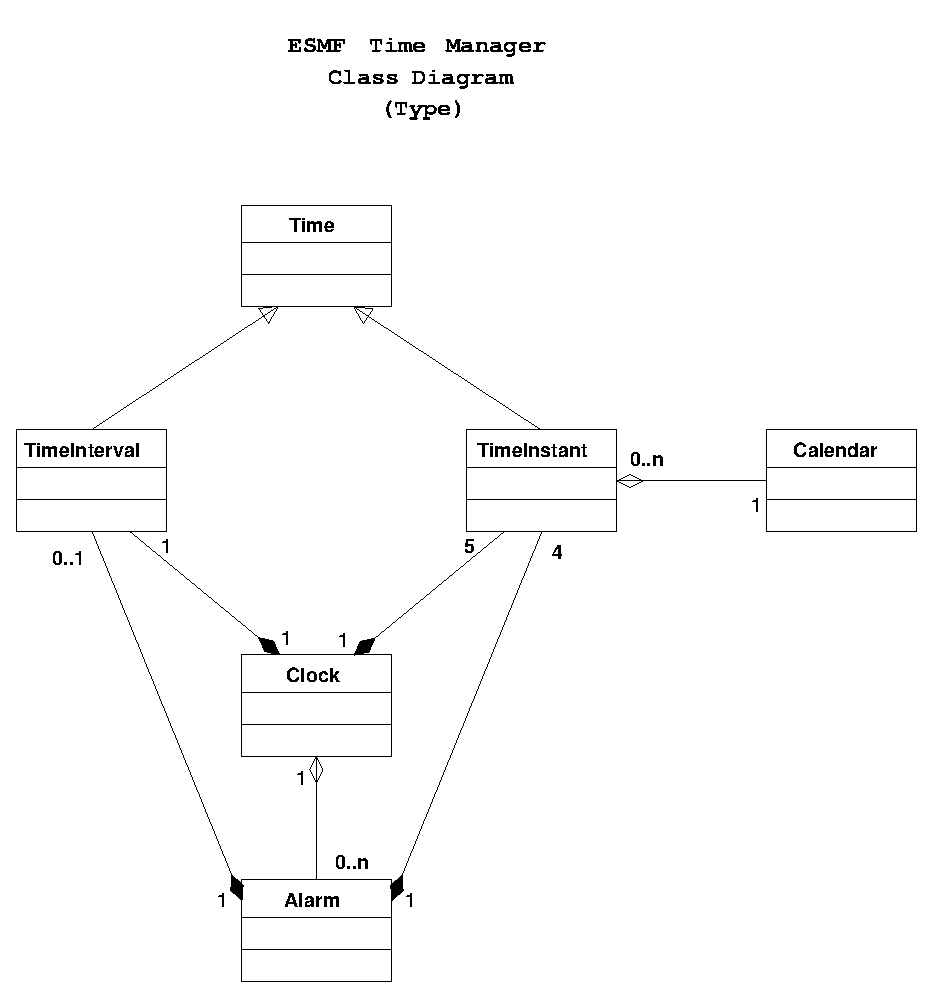
\includegraphics{TimeMgrClass.EPS}
   
Figure 1.  ESMF Time Manager Class Diagram
   
\end{center}

% $Id: TimeMgr_obj2.tex,v 1.1 2002/08/18 22:43:36 eschwab Exp $

%\section{Object Model}

Figure 2 shows the typical usage (instantiantion) of the Time Manager
within an application.  First, a calendar is created.  Then, time intervals
and time instants are created for clock usage and initialized as a time step,
start time, stop time and current time.  Similarly, a time interval and time 
instants are created and initialized for alarm usage.  Next, alarms are
created and intialized with the appropriate previously created time interval
and time instants.  Finally, a clock is created and initialized with its
corresponding time instants and time interval.  The clock is also associated
with the previously created calendar and alarms.  The clock is then ready
for timestepping and alarm checking.

\begin{center}
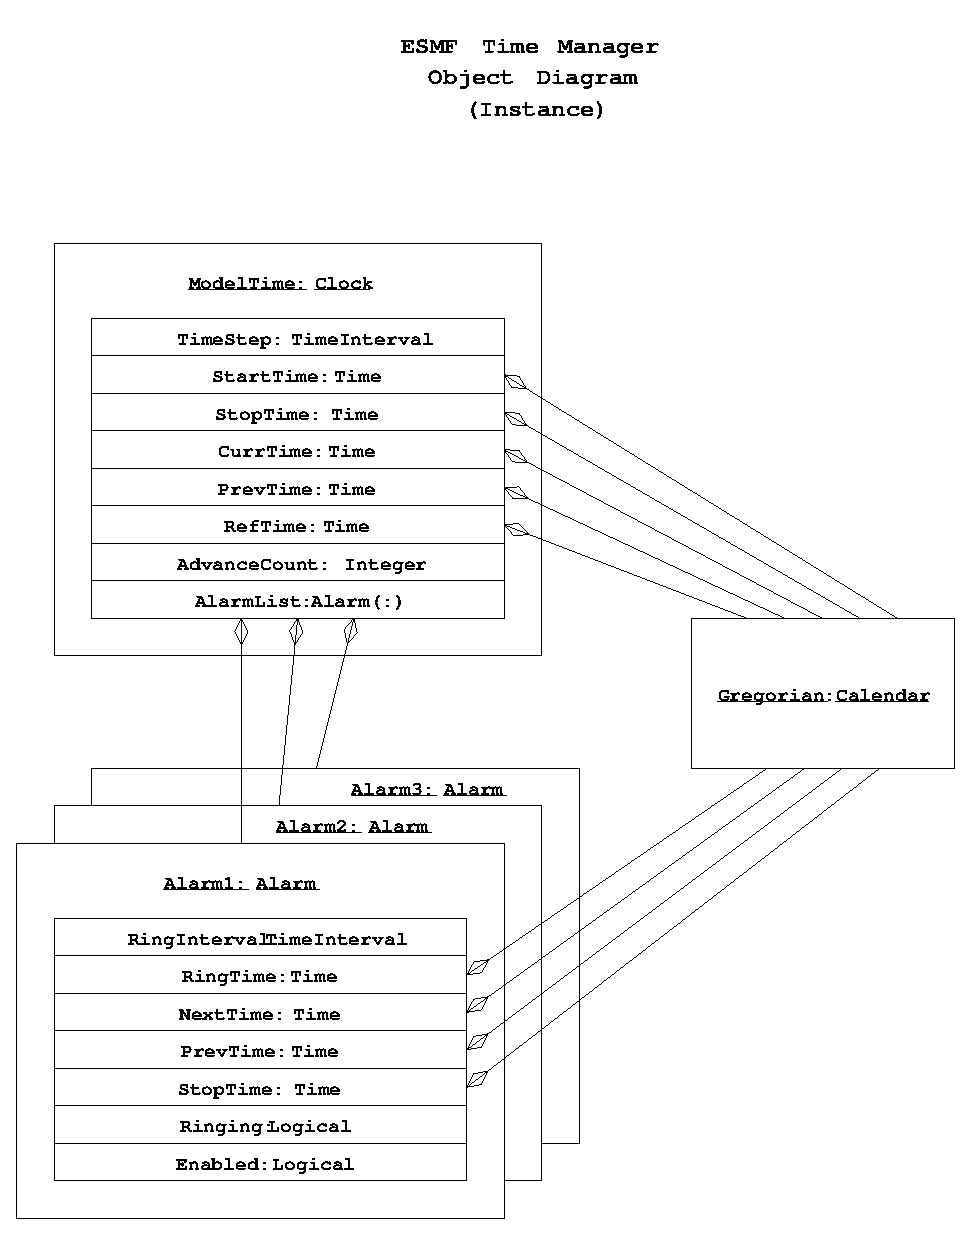
\includegraphics{TimeMgrObject.EPS}
   
Figure 2.  ESMF Time Manager Object Diagram
   
\end{center}

% $Id: TimeMgr_obj3.tex,v 1.2 2003/02/11 18:58:56 eschwab Exp $

%\section{Object Model}

Whereas Figures 1 and 2 are static structure UML diagrams, Figures 3, 4,  and
5 are dynamic behavioral UML diagrams.  Figure 3 shows how timestepping occurs
within an instance of Time Manager.  First, an ESM component invokes the
{\tt Advance()} method on its clock, named {\tt ModelTime} in this example.
In turn, {\tt ModelTime} increments its internal current time, called
{\tt CurrTime}.  A user only needs to know how to create a clock and invoke
its {\tt Advance()} method.  The implementation detail of actually performing
the increment is hidden from the user as it is encapsulated within the Time
Manager clock.

\begin{center}
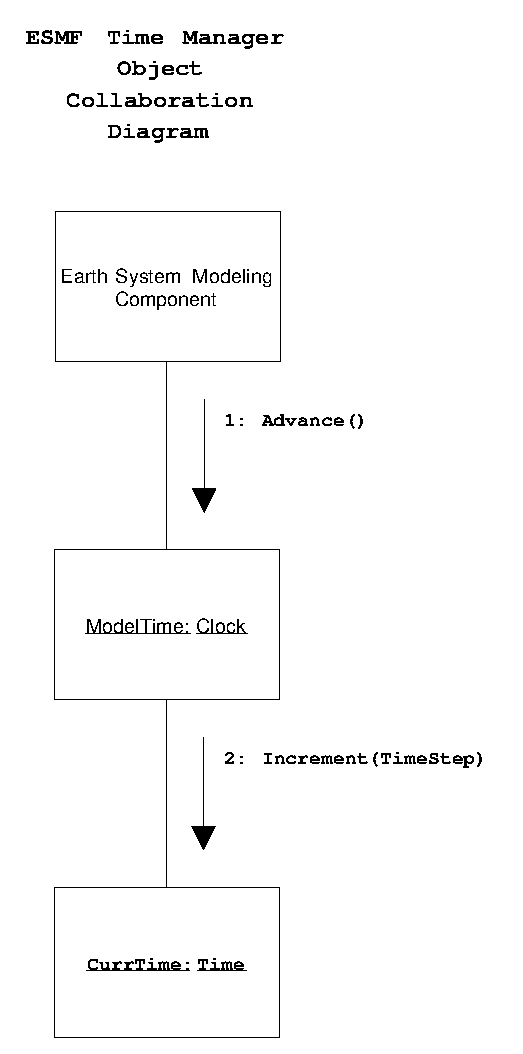
\includegraphics{TimeMgrOCD1.EPS}
   
Figure 3.  ESMF Time Manager Increment Model Time Scenario
   
\end{center}

% $Id: TimeMgr_obj4.tex,v 1.3 2004/01/27 23:05:07 eschwab Exp $

%\section{Object Model}

In Time Manager, all times are internally represented and operated on as
integer seconds and rational integer fractional seconds.  Specific date and
time formats are available to the user at the interface level, where
conversions are performed.  So the user gets/sets Time Manager's
{\tt TimeIntervals} and {\tt Time} instants in familiar units of year, month,
day, hour, minutes, seconds, and sub-seconds in their various required
combinations.  Figure 4 shows an example of a user's ESM component querying
its clock for the current time in (yy, mm, dd, h, m, s) format.  First the
model invokes the {\tt Get()} method on its clock's current time,
{\tt CurrTime}.  Next, internally (transparent to the user), {\tt CurrTime}
invokes the {\tt ConvertToDate()} method on its associated calendar, Gregorian.
Gregorian, in turn, performs the requisite conversion of {\tt CurrTime}'s
internal representation of time (integer seconds and fractional seconds)
to a Gregorian date.  Note that the calendar object is a single instance
shared among all Time instants, as previously shown in Figures 1 and 2.

\begin{center}
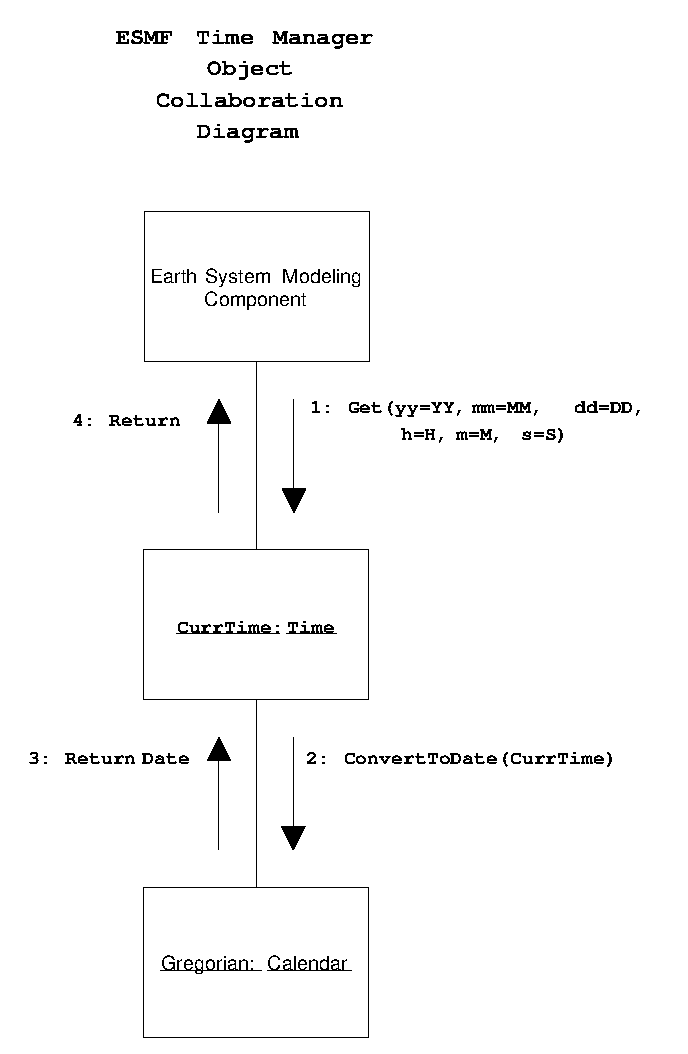
\includegraphics{TimeMgrOCD2.EPS}
   
Figure 4.  ESMF Time Manager Convert to Date Scenario
   
\end{center}

% $Id: TimeMgr_obj5.tex,v 1.1 2002/08/18 22:43:36 eschwab Exp $

%\section{Object Model}

In Figure 5, we see how a ESM component's clock checks its alarms.  After
the clock's current time is incremented (Model time stepped), the clock checks
all its alarms to see if its time for them to start or stop ringing.  All the
user needs to know is how to initialize the alarms and time step the clock;
the alarm checking happens internally "under the hood."
   
\begin{center}
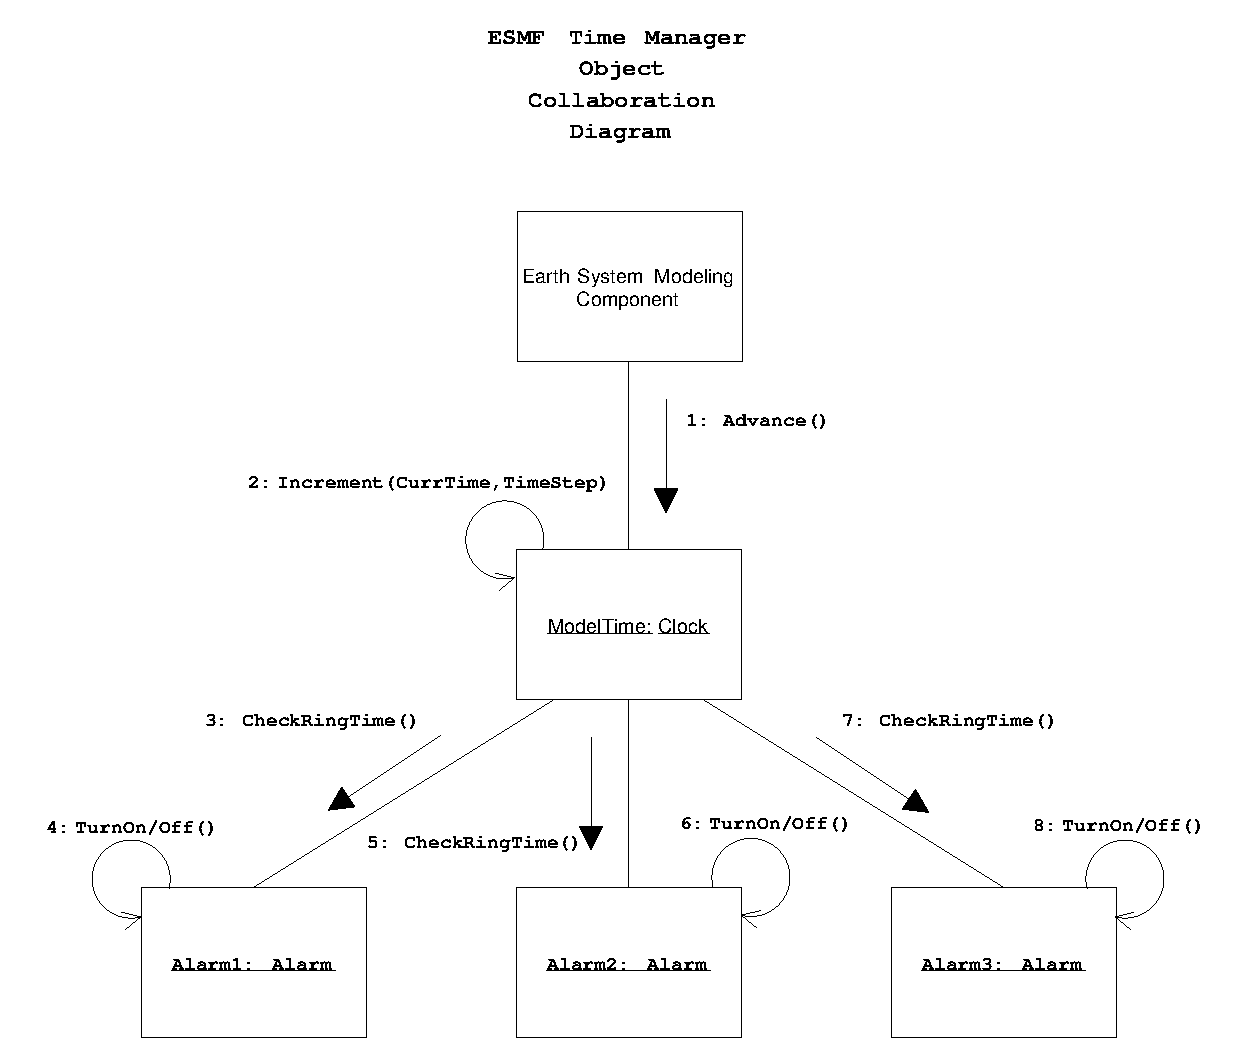
\includegraphics{TimeMgrOCD3.EPS}
   
Figure 5.  ESMF Time Manager Check Alarms Scenario
   
\end{center}


\section{Global Parameters and Definitions}
% $Id: TimeMgr_param.tex,v 1.3 2003/02/11 18:58:56 eschwab Exp $

Platform-independent specification of 64-bit integers are done via
compile-time constants in the F90 and C++ {\tt ESMF\_Base} classes as follows:

F90:
\begin{verbatim}
from ESMF_Base.F90:

    module ESMF_BaseMod
        .
        .
        .
        integer, parameter :: &
                     ESMF_IKIND_I8 = selected_int_kind(18), ! 18 decimal digits
        .
        .
        .
    end module ESMF_BaseMod
\end{verbatim}

C++:
\begin{verbatim}
from ESMC_Base.h:
.
.
.
#ifdef ESMF_IS_32BIT_MACHINE
.
.
.
  typedef long long ESMF_IKIND_I8;
.
.
.
#else // 64-bit or larger machine
.
.
.
  typedef long      ESMF_IKIND_I8;
.
.
.
#endif
.
.
.
\end{verbatim}


% ----------
% Time Class
% ----------

\section{Time Class Design}

\subsection{Description}
% $Id: time_desc.tex,v 1.1 2002/08/18 22:43:37 eschwab Exp $

The Time class is a base class which encapulates the core representation and
functionality of time for time intervals and time instances.


\subsection{Design}
\input{time_design}

\subsubsection{Class Definition}
% $Id: time_def.tex,v 1.1 2002/08/18 22:43:37 eschwab Exp $
\begin{verbatim}
        type ESMF_Time
            private
            sequence
                integer(int64) :: S     ! whole seconds
                integer(int32) :: Sn    ! fractional seconds, numerator
                integer(int32) :: Sd    ! fractional seconds, denominator
        end type
\end{verbatim}


\subsubsection{Restrictions}
\input{time_rest}

\section{Time Class F90 Interface}

\subsection{Use and Examples}
% $Id: time_fex.tex,v 1.1 2002/08/18 22:43:37 eschwab Exp $

The Time class is not intended for users; it is only used internally as a base
class for TimeInterval and TimeInstant.  The F90 definition for
TimeInstant is as follows:

\begin{verbatim}
        use ESMF_TimeMod

        type ESMF_TimeInstant
            private
            sequence
                type(ESMF_Time) :: time		! <== "inherits" base class
                integer :: calendar
                integer :: timezone
        end type
\end{verbatim}


\subsection{Parameters and Definitions}
%\input{time_fparam}

%\subsection{Class API}
\input{time_fapi}

\section{Time Class C++ Interface}

\subsection{Use and Examples}
% $Id: time_ccex.tex,v 1.1 2002/08/18 22:43:37 eschwab Exp $

The Time class is not intended for users; it is only used internally as a base
class for TimeInterval and TimeInstant.  The C++ definition for
TimeInstant are as follows:

\begin{verbatim}
class ESMC_TimeInstant : public ESMC_Time   // <== inherits base class
{
  private:

    ESMC_Calendar *Calendar;    // associated calendar
    int Timezone;               // Offset from GMT
};
\end{verbatim}


\subsection{Parameters and Definitions}
%\input{time_ccparam}

%\subsection{Class API}
\input{time_ccapi}

% -------------------
% Time Interval Class
% -------------------

\section{Time Interval Class Design}

\subsection{Description}
% $Id: time_interval_desc.tex,v 1.1 2002/08/18 22:43:37 eschwab Exp $

A TimeInterval inherits from the Time base class and is designed to represent
time deltas which are independent of any calendar.


\subsection{Design}
% $Id: time_interval_design.tex,v 1.1 2002/08/18 22:43:37 eschwab Exp $

TimeInterval inherits from the base class Time.  As such, it gains the core
representation of time as well as its associated methods.   TimeInterval
further specializes Time by adding shortcut methods to set and get a
TimeInterval in natural way with appropriate unit combinations, as per the
requirements.  The largest unit of time for a TimeInterval is a day, so a
TimeInterval is independent of any calendar.  This is in contrast with a
TimeInstant, which is calendar-dependent, since its largest units of time
are months and years.  TimeInterval also defines methods for multiplication
and division of TimeIntervals by integers, reals, fractions and other
TimeIntervals.  TimeInterval does not add any new attributes to Time.


\subsubsection{Class Definition}
% $Id: time_interval_def.tex,v 1.1 2002/08/18 22:43:37 eschwab Exp $
\begin{verbatim}
        type ESMF_TimeInterval 
            private
            sequence
                type(ESMF_Time) :: time
        end type
\end{verbatim}


\subsubsection{Restrictions}
%\input{time_interval_rest}

\section{Time Interval Class F90 Interface}

\subsection{Use and Examples}
$Id: time_interval_fex.tex,v 1.1 2002/08/18 22:43:37 eschwab Exp $

A TimeInterval will typically be used as a timestep for a clock or an alarm
interval.  The following shows how to create and initialize one in F90, based
on the example shown in Figure 2:

\begin{verbatim}
! use the TimeInterval Module
use ESMF_TimeIntervalMod

! create a TimeInterval
type(ESMF_TimeInterval) :: TimeStep

! initialize it to 3 days, 5 hours, 15 minutes, 30 seconds
call ESMF_TimeIntervalInit(TimeStep, D=3, H=5, M=15, S=30)

! pass it to a clock
call ESMF_ClockInit(ModelTime, TimeStep, ...)
\end{verbatim}


\subsection{Parameters and Definitions}
%\input{time_interval_fparam}

%\subsection{Class API}
\input{time_interval_fapi}

\section{Time Interval Class C++ Interface}

\subsection{Use and Examples}
%% $Id: time_interval_ccex.tex,v 1.1 2002/09/20 18:20:15 eschwab Exp $

A TimeInterval will typically be used as a timestep for a clock or an alarm
interval.  The following shows how to create and initialize one in C++, based
on the example shown in Figure 2:

\begin{verbatim}
// use the TimeInterval Class
#include <ESMF_TimeInterval.h>

// instantiate a TimeInterval
ESMC_TimeInterval TimeStep;

// initialize it to 3 days, 5 hours, 15 minutes, 30 seconds
TimeStep.Init("D:H:M:S", 3, 5, 15, 30);

// pass it to a clock
ModelTime.Init(&TimeStep, ...);
\end{verbatim}


\subsection{Parameters and Definitions}
%\input{time_interval_ccparam}

%\subsection{Class API}
\input{time_interval_ccapi}

% ------------------
% Time Instant Class
% ------------------

\section{Time Instant Class Design}

\subsection{Description}
% $Id: time_instant_desc.tex,v 1.1 2002/08/18 22:43:37 eschwab Exp $

A TimeInstant inherits from the Time base class and is designed to represent
a specific point in time which is dependent upon a calendar type.


\subsection{Design}
% $Id: time_instant_design.tex,v 1.1 2002/08/18 22:43:37 eschwab Exp $

TimeInstant inherits from the base class Time.  As such, it gains the core
representation of time as well as its associated methods.   TimeInstant
further specializes Time by adding shortcut methods to set and get a
TimeInstant in a natural way with appropriate unit combinations, as per the
requirements.  A TimeInstant is calendar-dependent, since its largest units
of time are months and years.  TimeInstant also defines special methods for
getting the day of the year, day of the week, middle of the month, and
synchronizing with a real-time clock.  TimeInstant adds its associated
Calendar and local Timezone attributes to Time.


\subsubsection{Class Definition}
% $Id: time_instant_def.tex,v 1.1 2002/08/18 22:43:37 eschwab Exp $
\begin{verbatim}
        type ESMF_TimeInstant
            private
            sequence
                type(ESMF_Time) :: time
                integer :: calendar
                integer :: timezone
        end type
\end{verbatim}


\subsubsection{Restrictions}
%\input{time_instant_rest}

\section{Time Instant Class F90 Interface}

\subsection{Use and Examples}
\input{time_instant_fex}

\subsection{Parameters and Definitions}
%\input{time_instant_fparam}

%\subsection{Class API}
\input{time_instant_fapi}

\section{Time Instant Class C++ Interface}

\subsection{Use and Examples}
%\input{time_instant_ccex}

\subsection{Parameters and Definitions}
%\input{time_instant_ccparam}

%\subsection{Class API}
\input{time_instant_ccapi}

% --------------
% Calendar Class
% --------------

\section{Calendar Class Design}

\subsection{Description}
% $Id: calendar_desc.tex,v 1.1 2002/08/18 22:43:36 eschwab Exp $

The Calendar class encapsulates the knowledge (attributes and behavior) of all
required calendar types:  Gregorian, Julian, no-leap, 360-day, generic, and
no-calendar.


\subsection{Design}
\input{calendar_design}

\subsubsection{Class Definition}
\input{calendar_def}

\subsubsection{Restrictions}
% $Id: calendar_rest.tex,v 1.1 2002/08/18 22:43:36 eschwab Exp $

Due to the requirement of only Earth modeling and the requirement for no
dynamic memory allocation, the number of months per year is hard-coded
at 12.  However, for easy modification, this is done via an F90 parameter
and a C++ \#define.  See the F90 and C++ "Parameters and Definitions" sections
below.


\section{Calendar Class F90 Interface}

\subsection{Use and Examples}
% $Id: calendar_fex.tex,v 1.1 2002/08/18 22:43:36 eschwab Exp $

A Calendar will be used as a reference for time instants.
The following shows how to create and initialize one in F90:

\begin{verbatim}
! use the Calendar Module
use ESMF_CalendarMod

! create a Calendar
type(ESMF_Calendar) :: Gregorian

! initialize it to be a Gregorian calendar
call ESMF_CalendarInit(Gregorian, ESMF_GREGORIAN)

! pass it to a time instant
call ESMF_TimeInstantInit(StartTime, ..., Gregorian)
\end{verbatim}


\subsection{Parameters and Definitions}
% $Id: calendar_fparam.tex,v 1.1 2002/08/18 22:43:36 eschwab Exp $

The Calendar class has one parameter which defines the number of months
in a year.  For different planetary bodies, this can be edited and
recompiled.

        integer, parameter :: MonthsPerYear = 12

If required, a future enhancement possibility would be to pass this as an
argument to the CalendarInit() method.  The advantage would be no source
code change required, but the disadvantage would be that it requires
dynamic memory allocation, which the requirements document disallows.


%\subsection{Class API}
\input{calendar_fapi}

\section{Calendar Class C++ Interface}

\subsection{Use and Examples}
%% $Id: calendar_ccex.tex,v 1.1 2002/09/20 18:20:11 eschwab Exp $

A Calendar will be used as a reference for time instants.
The following shows how to create and initialize one in C++:

\begin{verbatim}
// use the Calendar class
#include <ESMC_Calendar.h>

// create a Calendar
ESMC_Calendar Gregorian;

// initialize it to be a Gregorian calendar
Gregorian.Init(ESMC_GREGORIAN);

// pass it to a time instant
StartTime.Init(..., Gregorian);
\end{verbatim}


\subsection{Parameters and Definitions}
\input{calendar_ccparam}

%\subsection{Class API}
\input{calendar_ccapi}

% -----------
% Clock Class
% -----------

\section{Clock Class Design}

\subsection{Description}
% $Id: clock_desc.tex,v 1.1 2002/08/18 22:43:36 eschwab Exp $

The clock class encapsulates the essential ESM component requirement of
tracking and time-stepping model time.  It also checks associated alarms to
trigger their ringing state.


\subsection{Design}
\input{clock_design}

\subsubsection{Class Definition}
% $Id: clock_def.tex,v 1.1 2002/08/18 22:43:36 eschwab Exp $
\begin{verbatim}
        type ESMF_Clock
            private
            sequence
                type(ESMF_TimeInterval) :: TimeStep
                type(ESMF_TimeInstant)  :: StartTime
                type(ESMF_TimeInstant)  :: StopTime
                type(ESMF_TimeInstant)  :: RefTime
                type(ESMF_TimeInstant)  :: CurrTime
                type(ESMF_TimeInstant)  :: PrevTime
                integer(int32) :: AdvanceCount
                type(ESMF_Alarm), dimension(10) :: AlarmList
                integer :: ClockMutex
        end type
\end{verbatim}


\subsubsection{Restrictions}
\input{clock_rest}

\section{Clock Class F90 Interface}

\subsection{Use and Examples}
\input{clock_fex}

\subsection{Parameters and Definitions}
\input{clock_fparam}

%\subsection{Class API}
\input{clock_fapi}

\section{Clock Class C++ Interface}

\subsection{Use and Examples}
%% $Id: clock_ccex.tex,v 1.1 2002/09/20 18:20:12 eschwab Exp $

A Clock is the centerpiece of the Time Manager library, used to track time
in an ESM component.  The following shows how to create and initialize one
in C++, based on the example shown in Figure 2:

\begin{verbatim}
// use the Clock Class
#include <ESMC_Clock.h>

// create a Clock
ESMC_Clock ModelTime;

// create and initialize a calendar
ESMC_Calendar Gregorian;
Gregorian.Init(GREGORIAN);

// create and initialize clock time intervals and instants
ESMC_TimeInterval TimeStep;
ESMC_TimeInstant  StartTime, StopTime, RefTime;

TimeStep.Init(...);
StartTime.Init(..., Gregorian);
StopTime.Init(..., Gregorian);
RefTime.Init(..., Gregorian);

// initialize the clock
ModelTime.Init(TimeStep, StartTime, StopTime, RefTime);

// start time stepping
ModelTime.Advance();
\end{verbatim}


\subsection{Parameters and Definitions}
\input{clock_ccparam}

%\subsection{Class API}
\input{clock_ccapi}

% -----------
% Alarm Class
% -----------

\section{Alarm Class Design}

\subsection{Description}
% $Id: alarm_desc.tex,v 1.1 2002/08/18 22:43:36 eschwab Exp $

The Alarm class encapsulates the required alarm behavior, triggering its
ringing state on either a one-shot or repeating interval basis.


\subsection{Design}
% $Id: alarm_design.tex,v 1.1 2002/08/18 22:43:36 eschwab Exp $

The Alarm class contains TimeInstants and a TimeInterval to perform one-shot
and interval alarming.  A single TimeInterval holds the alarm interval if
used.  A TimeInstant is defined for the ring time, used for either the one-shot
alarm time or for the next interval alarm time.  TimeInstants are also
defined for next and previous ring times in keeping track of alarm intervals.
A TimeInstant for stop time defines when alarm intervals end.  If a one-shot
alarm is defined, only the ring time attribute is used, the others are not.
To keep track of alarm state, two logical attributes are defined, one for
ringing on/off, and the other for alarm enabled/disabled.  An alarm is 
enabled by default; if disabled by the user, it does not function at all.

The primary method is to check whether it is time to set the ringer, which
is called by the associated clock after performing a time step.  Other methods
are defined for getting the ringing state, turning the ringer on/off,
enabling/disabling the alarm, and getting/setting the time attributes
defined above.


\subsubsection{Class Definition}
% $Id: alarm_def.tex,v 1.1 2002/08/18 22:43:36 eschwab Exp $
\begin{verbatim}
        type ESMF_Alarm
            private
            sequence
                type(ESMF_TimeInterval) :: RingInterval
                type(ESMF_TimeInstant)  :: RingTime
                type(ESMF_TimeInstant)  :: NextRingTime
                type(ESMF_TimeInstant)  :: PrevRingTime
                type(ESMF_TimeInstant)  :: StopTime
                logical :: Ringing
                logical :: Enabled
                integer :: ID
                integer :: AlarmMutex
        end type
\end{verbatim}


\subsubsection{Restrictions}
%\input{alarm_rest}

\section{Alarm Class F90 Interface}

\subsection{Use and Examples}
% $Id: alarm_fex.tex,v 1.1 2002/08/18 22:43:36 eschwab Exp $

A Alarm is used in conjunction with a clock to ring at certain points in time.
The following shows how to create and initialize two in F90, based on the
example shown in Figure 2.  The first is a one-shot and the second is an
interval alarm.

\begin{verbatim}
! use the Alarm Module
use ESMF_AlarmMod

! create two Alarms
type(ESMF_Alarm) :: Alarm1, Alarm2

! Initialize one to be a one-shot
type(ESMF_TimeInstant) :: AlarmTime
call ESMF_TimeInstantInit(AlarmTime, YR=2002, MM=8, DD=30, Gregorian)
call ESMF_AlarmInit(Alarm1, RingTime=AlarmTime)

! Initialize other to ring on an interval
type(ESMF_TimeInterval) :: AlarmInterval
call ESMF_TimeIntervalInit(AlarmInterval, DD=1)
call ESMF_AlarmInit(Alarm2, RingInterval=AlarmInterval)

! Associate alarms with clock
call ESMF_ClockAddAlarm(ModelTime, Alarm1)
call ESMF_ClockAddAlarm(ModelTime, Alarm2)

! time step, clock reports active alarms in RingingAlarms list
call ESMF_ClockAdvance(ModelTime, RingingAlarms)

! process any active alarms
if (RingingAlarms(1) == Alarm1) then

   ! process Alarm1
   call ProcessAlarm1()

else if (RingingAlarms(2) == Alarm2) then

   ! process Alarm2
   call ProcessAlarm2()

   ! after processing alarms, turn off interval alarm to prepare for next
   !   ring time
   ESMF_AlarmTurnOff(Alarm2)

end if
\end{verbatim}


\subsection{Parameters and Definitions}
%\input{alarm_fparam}

%\subsection{Class API}
\input{alarm_fapi}

\section{Alarm C++ Interface}

\subsection{Use and Examples}
%\input{alarm_ccex}

\subsection{Parameters and Definitions}
%\input{alarm_ccparam}

%\subsection{Class API}
\input{alarm_ccapi}

\section{Review Status}

\noindent{\bf Design Review} \\

\begin{tabular}{r p{1.3in} p{2in}}
{\bf Review Date:} & <Date> \\ \\
{\bf Reviewers:}   & Reviewer           & <Institution> \\
                   & Reviewer           & <Institution> \\
                   & Reviewer           & <Institution>
\end{tabular}

\section{Glossary}
% $Id$

% USAGE NOTE:
%
% The first use of a term in the text of a document can be 
% linked to the corresponding glossary item using the item label.
% 
% For example,
%
% Original document text: code must include item1
%
% Linked to glossary:     code must include \htmlref{item1}{glos:item1}
%
% The link will appear in the html version of the document.
% The print version of the document will appear unchanged.

\begin{description}

\item [Normalized] \label{glos:Normalized} To limit the value of a given
time element to the next higher time element used.  For example, if
seconds and days are used, limit seconds to 86400, beyond which days
is incremented.  Similarly, if seconds and hours are used, limit seconds
to 3600.  For fractional seconds, if the numerator becomes >= denominator,
the whole seconds part is incremented and the numerator is reset to the
remainder.

\item [Bounded] \label{glos:Bounded} Synonymous with Normalize.

\end{description}


%\section{Bibliography}
\bibliography{comp} 
\bibliographystyle{plain}
\addcontentsline{toc}{section}{Bibliography}

\end{document}
